\documentclass[xcolor=x11names,compress]{beamer}
\usepackage[utf8]{inputenc}
\usepackage[spanish]{babel}
\usepackage{hyperref}
\hypersetup{colorlinks=true,linkcolor=white}
\usepackage{colortbl}
\usepackage{xcolor}
\usepackage{multirow}
\usepackage{fancyhdr}
\usepackage{graphicx}
\usepackage{listings}
\usepackage{framed}
\usepackage[version=0.96]{pgf}
\usepackage{tikz}
\usetikzlibrary{arrows,matrix,shapes,snakes,automata,backgrounds,petri}
\tikzstyle{information text}=[rounded corners, fill=gris]

\newcommand{\figuratikz}[3]
{
\begin{center}%
\begin{figure}[H]%
\begin{minipage}[H]{#1\columnwidth}%
\centering%
\begin{tikzpicture}{node distance=1.3cm,>=stealth',bend angle=45, auto}
{#3}
\end{tikzpicture}
\caption{#2}%
\end{minipage}%
\end{figure}%
\end{center}%
}

\definecolor{gris}{RGB}{243,243,243}
\definecolor{shadecolor}{RGB}{243,243,243}

\lstset{
  language=Python,
  basicstyle=\ttfamily\tiny,
  numbers=left,
  numberstyle=\tiny,
  stepnumber=1,
  numbersep=5pt,
  backgroundcolor=\color{gris},
  showspaces=false,
  showstringspaces=false,
  showtabs=false,
  frame=single,
  tabsize=2,
  captionpos=b,
  breaklines=true,
  breakatwhitespace=true,
  inputencoding=utf8,
  extendedchars=\true,
  keywordstyle=\color{blue}\bfseries\bf
  %code
  %fontstyle=\ttfamily
}

\renewcommand{\figurename}{Figura}

\newtheoremstyle{cuadrado}% name
  {3pt}%      Space above
  {3pt}%      Space below
  {\itshape}%         Body font
  {}%         Indent amount (empty = no indent, \parindent = para indent)
  {\itshape}% Thm head font
  {}%        Punctuation after thm head
  {0em}%     Space after thm head: " " = normal interword space;
        %       \newline = linebreak
  {}%         Thm head spec (can be left empty, meaning `normal')

\theoremstyle{cuadrado}
\newtheorem*{teo}{}


\newcommand{\slidesettitulo}{\textcolor{black}{Sensor para recopilación y visualización de información de seguridad en nodos de una red}}
\newcommand{\shorttitulo}{Security Sensor}
\newcommand{\authornombre}{Moisés Gautier Gómez}
\newcommand{\email}{moisesgautiergomez@correo.ugr.es}
\newcommand{\web}{Github: MGautier/security-sensor}
\newcommand{\institucion}{Universidad de Granada  \\ Escuela Técnica Superior de Ingenierías Informática y de Telecomunicación}
\newcommand{\tutor}{Gabriel Maciá Fernández}
\newcommand{\departamento}{Departamento de Teoría de la Señal, Telemática y Comunicaciones}
\newcommand{\titulacion}{Ingeniería en Informática}
\newenvironment{fondo}{\begin{teo}}{\end{teo}}



\definecolor{darkgray}{RGB}{237,236,236}
\definecolor{azuladwys}{RGB}{157,189,219}
\definecolor{azuladwys_version}{RGB}{174,208,239}
\definecolor{plata}{RGB}{145,143,144}


\usetheme{Ilmenau}

\setbeamertemplate{footline}{
\begin{tiny}
\setbeamercolor{foot1}{fg=black!70,bg=gray!10}
\setbeamercolor{foot2}{fg=gray,bg=gray!15}
\setbeamercolor{foot3}{fg=gray,bg=gray!10}
\setbeamercolor{foot4}{fg=black!70,bg=gray!20}
\setbeamercolor{foot5}{fg=gray,bg=gray!15}
\setbeamercolor{foot6}{fg=black,bg=gray!20}

%\setbeamercolor{foot1}{fg=azuladwys_version,bg=azuladwys_version}
%\setbeamercolor{foot2}{fg=azuladwys,bg=azuladwys}
%\setbeamercolor{foot3}{fg=azuladwys_version,bg=azuladwys_version}
%\setbeamercolor{foot4}{fg=azuladwys,bg=azuladwys}
%\setbeamercolor{foot5}{fg=azuladwys,bg=azuladwys}
%\setbeamercolor{foot6}{fg=black,bg=gray!20}

% taken from theme infolines and adapted
  \leavevmode%
  \hbox{%
  \begin{beamercolorbox}[wd=.35\paperwidth,ht=2.25ex,dp=1ex,center]{foot1}%
  %\fontsize{5}{5}\selectfont
  \shorttitulo
  \end{beamercolorbox}%
  \begin{beamercolorbox}[wd=.1\paperwidth,ht=2.25ex,dp=1ex,center]{foot2}
  \end{beamercolorbox}%
    \begin{beamercolorbox}[wd=.05\paperwidth,ht=2.25ex,dp=1ex,center]{foot3}
  \end{beamercolorbox}%
    \begin{beamercolorbox}[wd=.25\paperwidth,ht=2.25ex,dp=1ex,center]{foot4}%
  %\fontsize{5}{5}\selectfont
  \web
  \end{beamercolorbox}%
  \begin{beamercolorbox}[wd=.05\paperwidth,ht=2.25ex,dp=1ex,center]{foot5}
  \end{beamercolorbox}%
  \begin{beamercolorbox}[wd=.2\paperwidth,ht=2.25ex,dp=1ex,right]{foot6}%
	\insertframenumber{} / \inserttotalframenumber \hspace*{2ex} 
  \end{beamercolorbox}}%
  \vskip0pt%
\end{tiny}
\vskip10pt
}


%\setbeamertemplate{footline}{}
\setbeamertemplate{navigation symbols}{} %Elimina los iconos que permiten la navegación en el documento

\usecolortheme[named=darkgray]{structure}
\usefonttheme{professionalfonts}
\useoutertheme{miniframes}

\title{\slidesettitulo}
\author{Alumno: \authornombre \newline \newline \email \newline \newline Director: \tutor \newline Titulación: \titulacion}
\institute{\departamento \newline \newline \institucion}
\date{ }
\setcounter{subsection}{0}

\begin{document}
\scriptsize{

\frame{\titlepage
  
}
\section{Presentación}
\subsection{Motivación y objetivos}

\frame{\frametitle{\textcolor{black}{Motivación y objetivos}}

El objetivo principal del proyecto es desarrollar un software que permita recopilar y visualizar la información generada por las aplicaciones de monitorización y control de seguridad que se ejecutan en una máquina. \newline


La motivación del mismo surge fruto de la necesidad de monitorizar una red corporativa a través de un mecanismo de gestión automatizada de eventos. Los pasos para la realización de este sistema se han modularizado y dividido en diferentes etapas que se acometarán como un todo dentro del proyecto de investigación VERITAS (http://nesg.ugr.es/veritas/) del Network Engineering \& Security Group (NESG - http://nesg.ugr.es/) perteneciente al área de Ingeniería Telemática de la Universidad de Granada. \newline

}

\subsection{Veritas}

\frame{\frametitle{\textcolor{black}{VERITAS}}

\begin{figure}[H]
  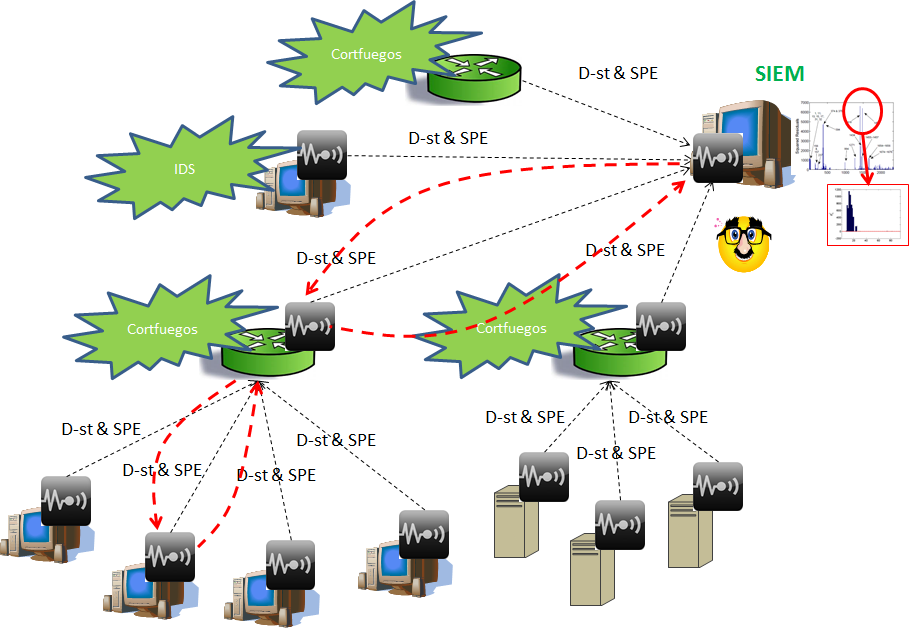
\includegraphics[scale=.25]{veritas.png}
\end{figure}
  \center{Figura - Nodos de una red - VERITAS}

}

\section{Tecnologías}

\subsection{Desarrollo Backend}
\frame{\frametitle{\textcolor{black}{Desarrollo Backend}}

\center{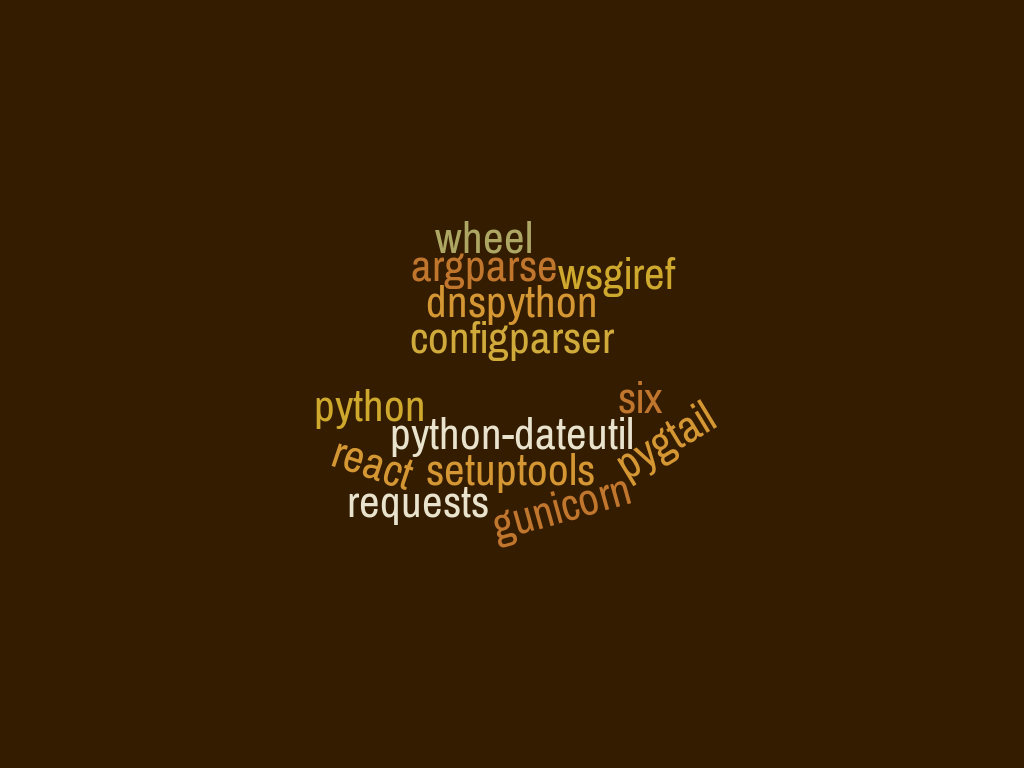
\includegraphics[scale=.24]{wordcloud.png}}

}

\subsection{Desarrollo interfaz web}
\frame{\frametitle{\textcolor{black}{Desarrollo interfaz web}}

\center{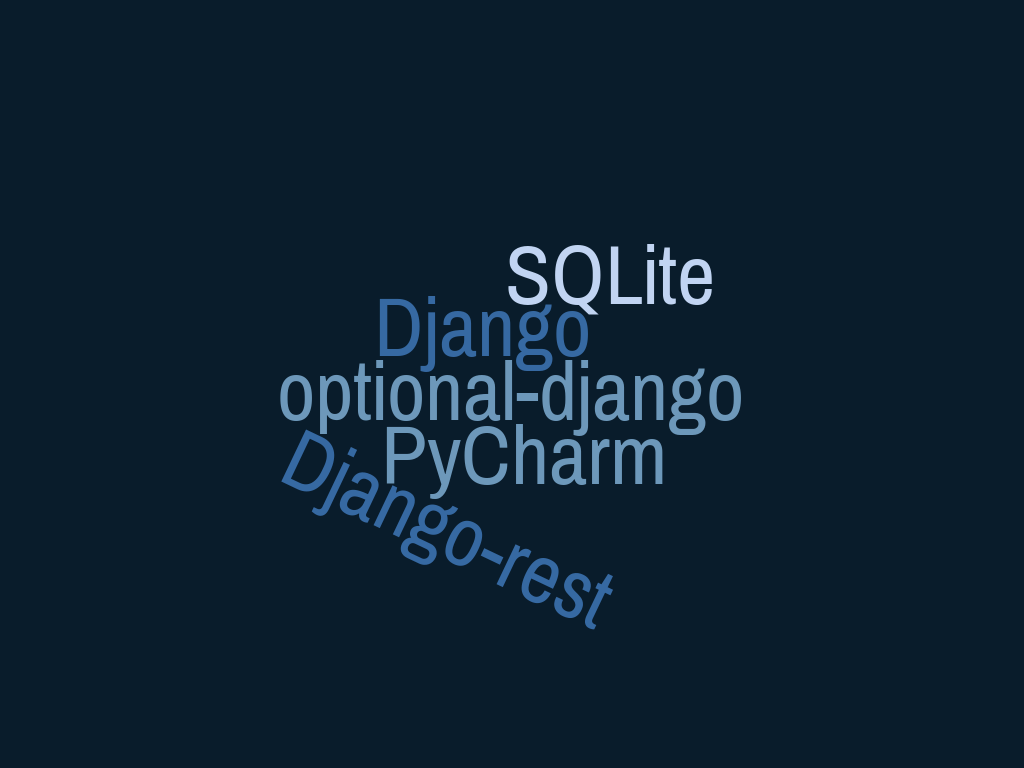
\includegraphics[scale=.24]{wordcloud-1.png}}

}

\subsection{Gestión de proyecto}
\frame{\frametitle{\textcolor{black}{Gestión de proyecto}}

\center{
\includegraphics[scale=.24]{wordcloud-2.png}}

}

\subsection{Servicios web}
\frame{\frametitle{\textcolor{black}{Servicios web}}

\center{
\includegraphics[scale=.24]{wordcloud-3.png}}

}

\subsection{Eventos y recolección}
\frame{\frametitle{\textcolor{black}{Eventos y recolección}}

\center{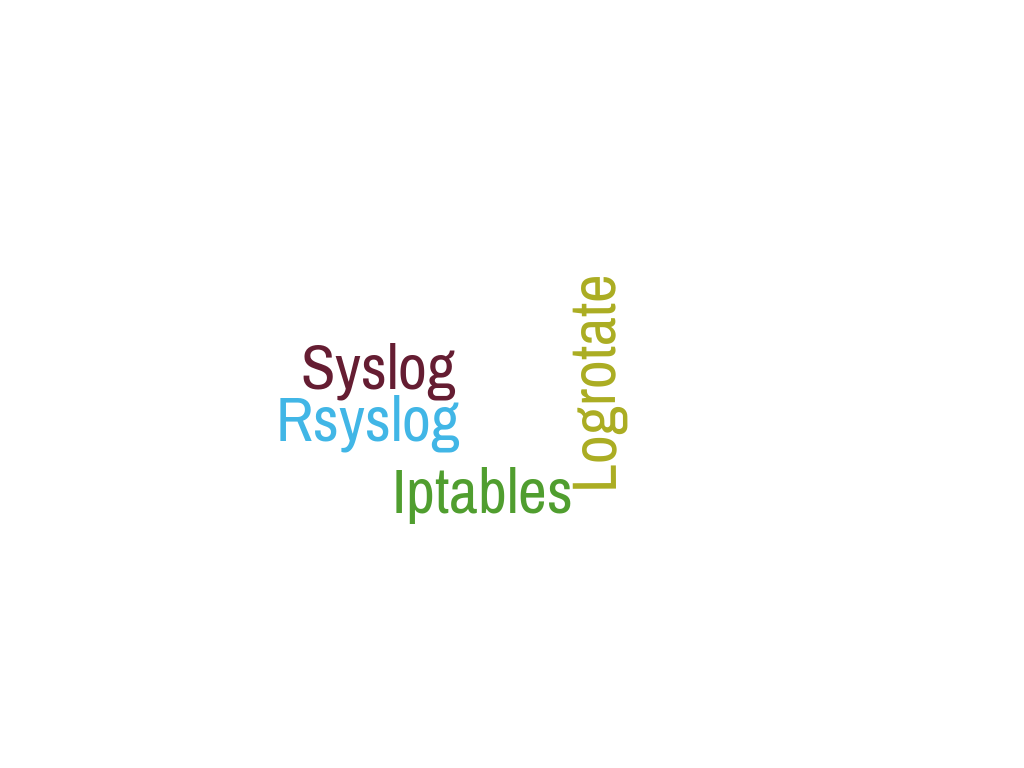
\includegraphics[scale=.24]{wordcloud-4.png}}

}

\subsection{Bibliotecas gráficas}
\frame{\frametitle{\textcolor{black}{Bibliotecas gráficas / javascript}}

\center{
\includegraphics[scale=.24]{wordcloud-5.png}}

}

\section{Arquitectura}

\subsection{Backend}

\frame{\frametitle{\textcolor{black}{Clases del sistema}}

  \hspace*{-.25in}{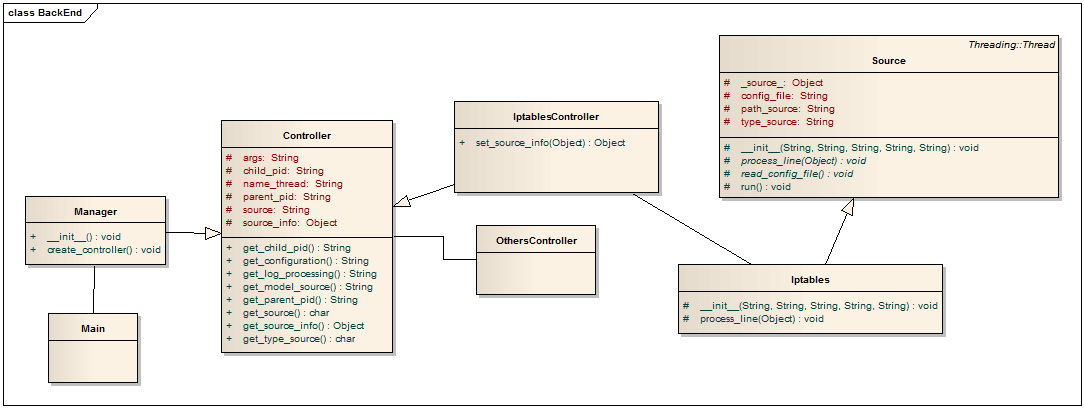
\includegraphics[scale=.42]{back-end.png}}\\
  \center{Figura - Diagrama de clases Backend}

}

\subsection{Frontend}

\frame{\frametitle{\textcolor{black}{Clases del sistema}}

  \center{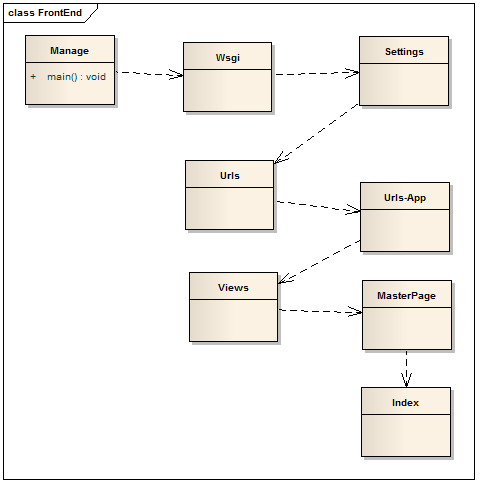
\includegraphics[scale=.5]{front-end.png}}\\
  Figura - Diagrama de clases Frontend

}

\frame{\frametitle{\textcolor{black}{Workflow Django}}
  \center{
    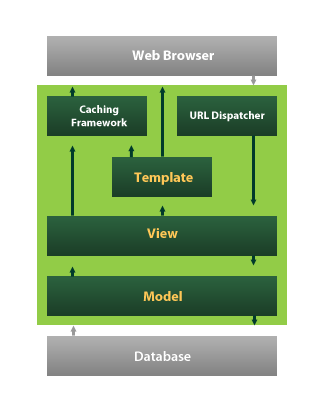
\includegraphics[scale=.4]{django-workflow.png}
  }
  http://mytardis.readthedocs.io/en/3.5/\_images/DjangoArchitecture-JeffCroft.png
}

\subsection{Modelo}

\frame{\frametitle{\textcolor{black}{Base de datos}}

\center{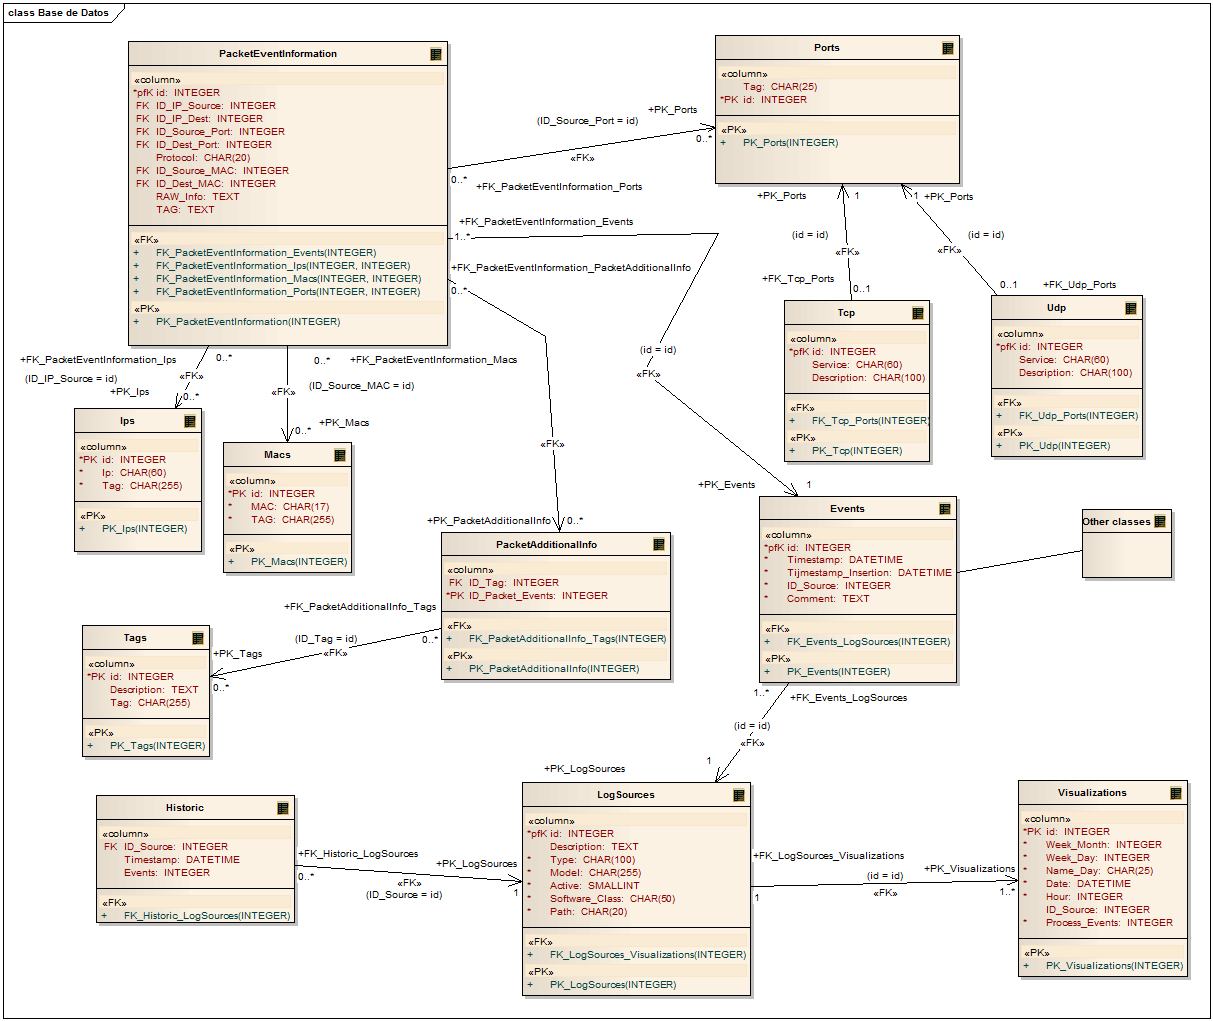
\includegraphics[scale=.25]{bd.png}}

}

\section{Implementación}

\subsection{Rsyslog}
\begin{frame}[fragile]
  \frametitle{\textcolor{black}{Rsyslog}}

  \begin{lstlisting}[language=bash]
    #
    # Use traditional timestamp format.
    # To enable high precision timestamps, comment out the following line.
    #
    #$ActionFileDefaultTemplate RSYSLOG_TraditionalFileFormat

    #
    # Set the default permissions for all log files.
    #
    $FileOwner root
    $FileGroup adm
    $FileCreateMode 0644
    $DirCreateMode 0755
    $Umask 0022

    # IPTABLES

    :msg,contains,"IPTMSG= " -/var/log/iptables.log
    :msg,regex,"^\[ *[0-9]*\.[0-9]*\] IPTMSG= " -/var/log/iptables.log
    :msg,contains,"IPTMSG= " ~

  \end{lstlisting}
  
  \hspace*{1in}{Figura - Configuración de iptables para Rsyslog}
\end{frame}

\subsection{Logrotate}

\begin{frame}[fragile]
  \frametitle{\textcolor{black}{Logrotate}}

  \begin{lstlisting}[language=bash]
    /var/log/iptables.log
    {
      rotate 7
      daily
      missingok
      notifempty
      delaycompress
      compress
      postrotate
      invoke-rc.d rsyslog restart > /dev/null
      endscript
    }
  \end{lstlisting}
  \hspace*{1in}{Figura - Configuración de iptables para Logrotate}
\end{frame}

\subsection{Iptables}

\begin{frame}[fragile]
  \frametitle{\textcolor{black}{Iptables}}

  \begin{lstlisting}[language=bash]
    # Generated by iptables-save v1.4.21 on Mon Jan 25 20:37:18 2016
    *filter
    :INPUT ACCEPT [0:0]
    :FORWARD ACCEPT [0:0]
    :OUTPUT ACCEPT [0:0]
    -A INPUT -d 127.0.0.1/32 -p icmp -m icmp --icmp-type 8 -m state --state NEW,RELATED,ESTABLISHED -j LOG --log-prefix "IPTMSG=Connection ICMP "
    -A INPUT -d 127.0.0.1/32 -p icmp -m icmp --icmp-type 8 -m state --state NEW,RELATED,ESTABLISHED -j DROP
    -A INPUT -p tcp -m tcp --dport 22 -j LOG --log-prefix "IPTMSG=Connection SSH "
    -A INPUT -p tcp -m tcp --dport 22 -j DROP
    COMMIT
  \end{lstlisting}
  \hspace*{1in}{Figura - Configuración reglas iptables}
\end{frame}

\subsection{Eventos}

\begin{frame}[fragile]
  \frametitle{\textcolor{black}{Eventos de Iptables}}

\begin{lstlisting}[language=bash, breaklines=true]
2016-07-03T17:03:35.664324+02:00 debian kernel: [23337.363387] IPTMSG=Connection SSH IN=lo OUT= MAC=00:00:00:00:00:00:00:00:00:00:00:00:08:00 SRC=127.0.0.1 DST=127.0.0.1 LEN=60 TOS=0x00 PREC=0x00 TTL=64 ID=39454 DF PROTO=TCP SPT=47706 DPT=22 WINDOW=43690 RES=0x00 SYN URGP=0
2016-07-03T17:03:37.668326+02:00 debian kernel: [23339.369692] IPTMSG=Connection SSH IN=lo OUT= MAC=00:00:00:00:00:00:00:00:00:00:00:00:08:00 SRC=127.0.0.1 DST=127.0.0.1 LEN=60 TOS=0x00 PREC=0x00 TTL=64 ID=39455 DF PROTO=TCP SPT=47706 DPT=22 WINDOW=43690 RES=0x00 SYN URGP=0
\end{lstlisting}
\hspace*{.3in}{Figura - Log capturado y almacenado por rsyslog en /var/log/iptables.log}
\end{frame}

\subsection{Pygtail}

\begin{frame}[fragile]
  \frametitle{\textcolor{black}{Correlación}}
  \lstinputlisting{codigo-4.py}
  \hspace*{.5in}{Figura - Instancia de la clase Pygtail y lectura de las líneas del log}
\end{frame}
}

\subsection{main.py}

\begin{frame}[fragile]
  \frametitle{\textcolor{black}{Main}}

\begin{lstlisting}[breaklines=true]

import signal
import os
import manager
import re


if __name__ == "__main__":

    # Instanciamos la clase Manager para la ejecucion de las distintas fuentes
    manager_obj = manager.Manager()

    # Obtenemos la instancia de la fuente iptables para su ejecucion devuelta por el controlador asociado
    iptables = manager_obj.create_controller('iptables')

    # Si establecemos iptables como un pid independiente tendremos que hacer uso de fork para esto y
    # asi el hilo Main sera sobre el cual se haran los operaciones

    if not iptables.get_child_pid() == iptables.get_parent_pid():
        threads = {'Main thread': iptables.get_parent_pid(), 'Thread-1': iptables.get_child_pid()}
    else:
        threads = {'Main thread': iptables.get_parent_pid()}

\end{lstlisting}
\end{frame}

\section{Pruebas}

\subsection{Evaluación}

\begin{frame}[fragile]
\frametitle{\textcolor{black}{Test de integridad - Events}}
\lstinputlisting{codigo-9-events-class.py}
\hspace*{.75in}{Figura - Test unitario clases del modelo - Events}
\end{frame}

\begin{frame}[fragile]
\frametitle{\textcolor{black}{Test de integridad - Events}}
\lstinputlisting{codigo-9-events-test-events-timestamp.py}
\hspace*{.75in}{Figura - Método de la clase Test test\_events\_timestamp}
\end{frame}

\section{Conclusiones}

\frame{\frametitle{\textcolor{black}{Conclusión}}

Durante la realización de éste proyecto, se han conseguido los siguientes resultados:

\begin{itemize}
\item Comprender el funcionamiento de los servicios del sistema: rsyslog, syslog, logrotate, nginx.
\item Comprender el funcionamiento del firewall del kernel, Iptables.
\item Desarrollar una solución software usando el lenguaje de programación Python.
\item Desarrollar una solución software, para sistemas web, usando el framework Django.
\item Manipulación de bases de datos relacionales usando un modelo orientado a objetos (ORM) proporcionado por el framework de desarrollo.
\item Diseñar el prototipo base para los sensores de recopilación de información de seguridad.
\item Diseñar una interfaz web donde el usuario pueda visualizar la información que el sensor ha analizado.
\item Despliegue de la aplicación en un servidor web en la nube para realizar demostraciones de la herramienta (Digital Ocean).
\item Documentar todo el proceso de realización del proyecto.
\end{itemize}
}

\section{Demo}

\frame{\frametitle{\textcolor{black}{Demostración}}

  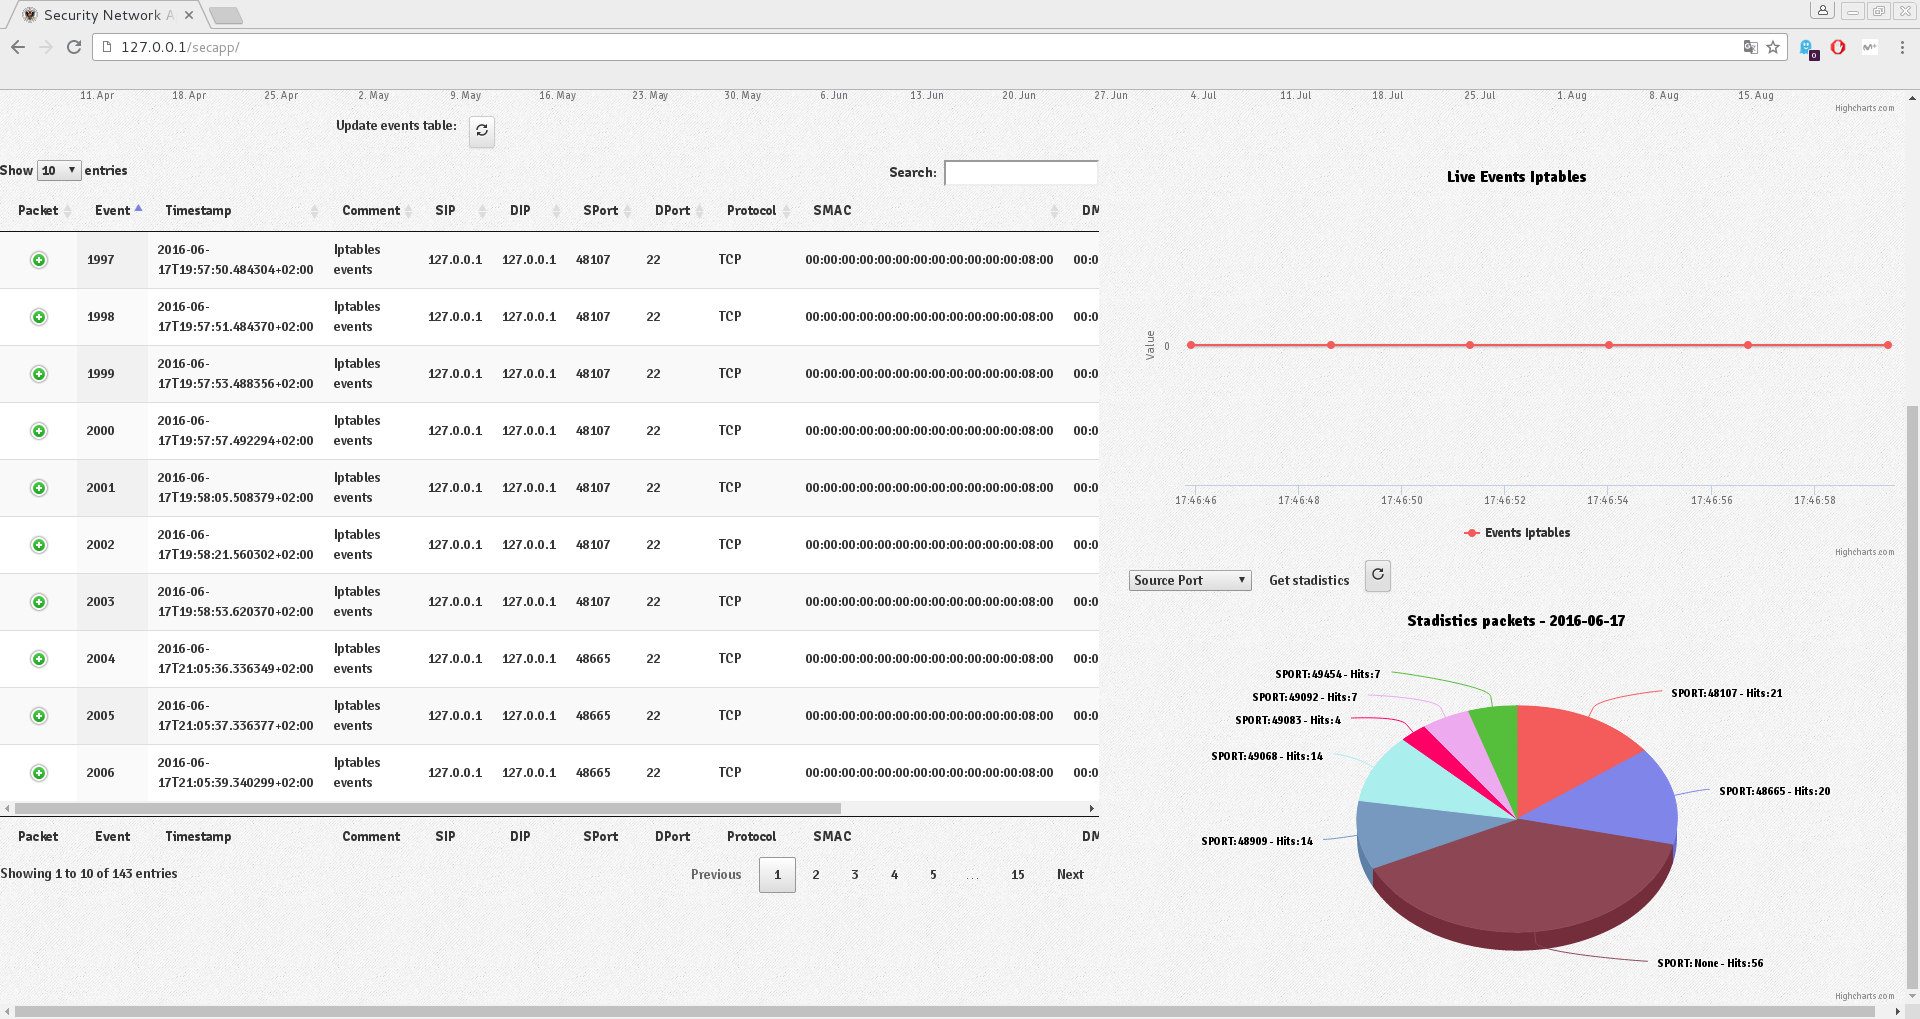
\includegraphics[scale=.15]{web_5.png}
}

\frame{\frametitle{\textcolor{black}{Final}}
{
\begin{center}
\huge{¿Preguntas?}
\begin{figure}[H]
  
\includegraphics[width=2cm]{question.png}
\end{figure}
\end{center}
\scriptsize{Figura - http://ph03nyx.deviantart.com/}



Para más información: https://github.com/MGautier/security-sensor \newline

}
}
\end{document}

